\section{Auswertung}
\subsection{Wheatstonesche Brücke}
Mithilfe der Wheatstonesche Brücke wurden die Widerstände \glqq Wert 13\grqq{} und \glqq Wert 14\grqq{} ermittelt. Zu berechnung dieser wurde die Formel (\ref{eqn:r_x}) genutzt.
Wie bereits in der Durchführung erwähnt wurden zwei Messreihen mit unterscheidlichen Widerständen zum selben unbekannten Widerstand durchgeführt. Der ermittelte Wert wurde dann gemittelt. In der folgenden Tabelle sind diese 
nochmal aufgelistet:

\begin{table}
\centering
\begin{tabular}{c c c c}
\toprule
{$R_2 \mathbin{/} \si{\ohm} $} & {$R_3 \mathbin{/} \si{\ohm} $} &{$R_4 \mathbin{/} \si{\ohm} $} & {$R_X \mathbin{/} \si{\ohm} $}\\
\midrule
664  &   317.5 &  682.5 & 308.89 \\
1000 &   239   &  761   & 314.06\\
\bottomrule
\end{tabular}
\caption{Daten für Wert 13}
\label{tab:wert13}
\end{table}

\begin{table}
\centering
\begin{tabular}{c c c c}
\toprule
{$R_2 \mathbin{/} \si{\ohm} $} & {$R_3 \mathbin{/} \si{\ohm} $} &{$R_4 \mathbin{/} \si{\ohm} $} & {$R_X \mathbin{/} \si{\ohm} $}\\
\midrule
664  &   573.5 &  426.5 & 892.86   \\
1000 &   471   &  529   & 890.36   \\
\bottomrule
\end{tabular}
\caption{Daten für Wert 14}
\label{tab:wert14}
\end{table}

Gemittelt ergibt dies für die Widerstände, dass:

\begin{align*}
\text{Wert} 13 &= 311.475 \, \si{\ohm}, \\
\text{Wert} 14 &= 891.61 \, \si{\ohm} \\
\end{align*}

ist.

\subsection{Kapazitätsmessbrücke}

Bei der Kapazitätmessbrücke wird der Ohmische Widerstand und die Kapazität eines Kondensators durch die Formeln (\ref{eqn:r_x}) und (\ref{eqn:c_x}) berechnet. Auch hier wurden die 
Widerstände variiert und mehrere Messungen durchgeführt um eine höhere Genauigkeit zu haben.
In den Tabellen (\ref{tab:ab8}) und (\ref{tab:ab9}) sind die Messwerte aufgeführt.

Mit diesen Werten lassen sich die Kapazitäten und Widerstände von Wert 8 bestimmen zu:

\begin{align*}
\text{Messung}1:& R_X = 570.62 \si{\ohm};  & C_X =  6.921\,  10\textsuperscript{-7}  \si{\farad}\\
\text{Messung}2:& R_X = 572.52 \si{\ohm};  & C_X = 5.465 \, 10\textsuperscript{-7}  \si{\farad}\\
\text{Messung}3:& R_X = 572.15 \si{\ohm};  & C_X = 1.229 \, 10\textsuperscript{-6}  \si{\farad}\\
\text{Gemittelt}:& R_X = 571.763 \si{\ohm};& C_X = 8.225 \, 10\textsuperscript{-7}  \si{\farad}\\
\end{align*}

und Wert 9 bestimmen zu:

\begin{align*}
\text{Messung}1:&  R_X = 486.97 \si{\ohm};& C_X =  4.702 \,  10\textsuperscript{-7}   \si{\farad}\\
\text{Messung}2:&  R_X = 485.63 \si{\ohm};& C_X = 3.698  \, 10\textsuperscript{-7}   \si{\farad}\\
\text{Messung}3:&  R_X = 488.10 \si{\ohm};& C_X = 8.278  \, 10\textsuperscript{-7}   \si{\farad}\\
\text{Gemittelt}:& R_X= 486.90 \si{\ohm};& C_X = 5.559 \,  10\textsuperscript{-7}   \si{\farad}\\
\end{align*}

Jedoch sind die Widerstände mit einem Fehler von $\pm 3\% $behaftet.

\subsection{Induktivitätsmessbrücke}

Bei der Induktivitätsmessbrücke wird der Verlustwiderstand, sowie die Induktivität einer Spule durch mehrmalige Messungen berechnet. Dazu wird die Formeln ie Formeln (\ref{eqn:r_x}) 
und (\ref{eqn:l_x}) genutzt. Die Tabellen aus denen die Messwerte entnommen werden sind (\ref{tab:ac10}) und (\ref{tab:ac18}).

Mit diesen Werten lassen sich die Induktivitäten und Widerstände von Wert 10 bestimmen zu:

\begin{align*}
\text{Messung}1:& R_X = 491.74 \si{\ohm};& L_X =  0.1595 \,  \si{\henry}\\
\text{Messung}2:& R_X = 399.00 \si{\ohm};& L_X =  0.1407 \,   \si{\henry}\\
\text{Messung}3:& R_X = 436.47 \si{\ohm};& L_X =  0.1412 \,    \si{\henry}\\
\text{Gemittelt}:& R_X= 442.40 \si{\ohm};& L_X = 8.225   \, \si{\henry}\\
\end{align*}

und Wert 18 bestimmen zu:

\begin{align*}
\text{Messung}1:& R_X = 372.00 \si{\ohm};& L_X =  0.0502 \si{\henry}\\
\text{Messung}2:& R_X = 157.79 \si{\ohm};& L_X =  0.0221 \si{\henry}\\
\text{Messung}3:& R_X = 362.66 \si{\ohm};& L_X =  0.0506 \si{\henry}\\
\text{Gemittelt}:& R_X=297.48 \si{\ohm};&  L_X =  0.0410 \si{\henry}\\
\end{align*}

Jedoch sind die Widerstände mit einem Fehler von $\pm 3\% $behaftet.


\subsection{Induktivitätsmessung mittels Maxwell-Brücke}

Hier werden die Spulen nochmal mittels der Maxwell-Brücke nochmal berechnet. Hierfür werden die Formeln  (\ref{eqn:r_x}) und (\ref{eqn:l_xM}) verwendet.
Jedoch sind die Größen $R_3$ und $R_4$ mit einem Fehler $\pm 3\%$ behaftet. Aus den Tabellen (\ref{tab:ad10}) und (\ref{tab:ad18}) folgt (mit $C_4 = 399 \si{\nano\farad} $) für Wert 10:

\begin{align*}
\text{Messung}1:& R_X =  41.86 \pm 2.51  \si{\ohm};& L_X =  0.0138 \, \si{\henry}\\
\text{Messung}2:& R_X = 418.90 \pm 25.13 \si{\ohm};& L_X =  0.1386 \, \si{\henry}\\
\text{Messung}3:& R_X = 414.90 \pm 24.89 \si{\ohm};& L_X =  0.1372 \, \si{\henry}\\
\text{Gemittelt}:& R_X= 416.90 \pm 25.01 \si{\ohm};& L_X =  0.1379 \, \si{\henry}\\ 
\end{align*}

und Wert 18:

\begin{align*}
\text{Messung}1:& R_X = 36.88  \pm 2.21  \si{\ohm};& L_X =  0.0051 \, \si{\henry}\\
\text{Messung}2:& R_X = 367.20 \pm 22.03 \si{\ohm};& L_X =  0.0511 \, \si{\henry}\\
\text{Messung}3:& R_X = 364.44 \pm 21.86 \si{\ohm};& L_X =  0.0506 \, \si{\henry}\\
\text{Gemittelt}:& R_X= 365.82 \pm 21.95 \si{\ohm};& L_X =  0.0509 \, \si{\henry}\\
\end{align*}

Da die Werte der ersten Messung erheblich von den beiden anderen Messugnen abweichen wurden diese in die Mittelwertbildung nicht mit einbezogen.


\subsection{Wien-Robinson-Brücke}

Hier wurde die Frequenzabhängigkeit der Brückenspannung der Wien-Robinson-Brücke im Bereich 20 ≤ $\omega$ ≤ 30 000 Hz untersucht. 
In der folgenden Grafik ist der Quotient aus $U_\text{Br}$ und $U_\text{S}$ gegen $\omega/\omega_0$ nach (\ref{eqn:omega0}) und (\ref{eqn:omega}) in blau aufgetragen.
Zusätzlich wurde in grün gestrichelt die theoretisch erwartete Werte nach der Wurzel (\ref{eqn:betragub2}) auf der Kurve aufgetragen.
\begin{figure}
    \centering
    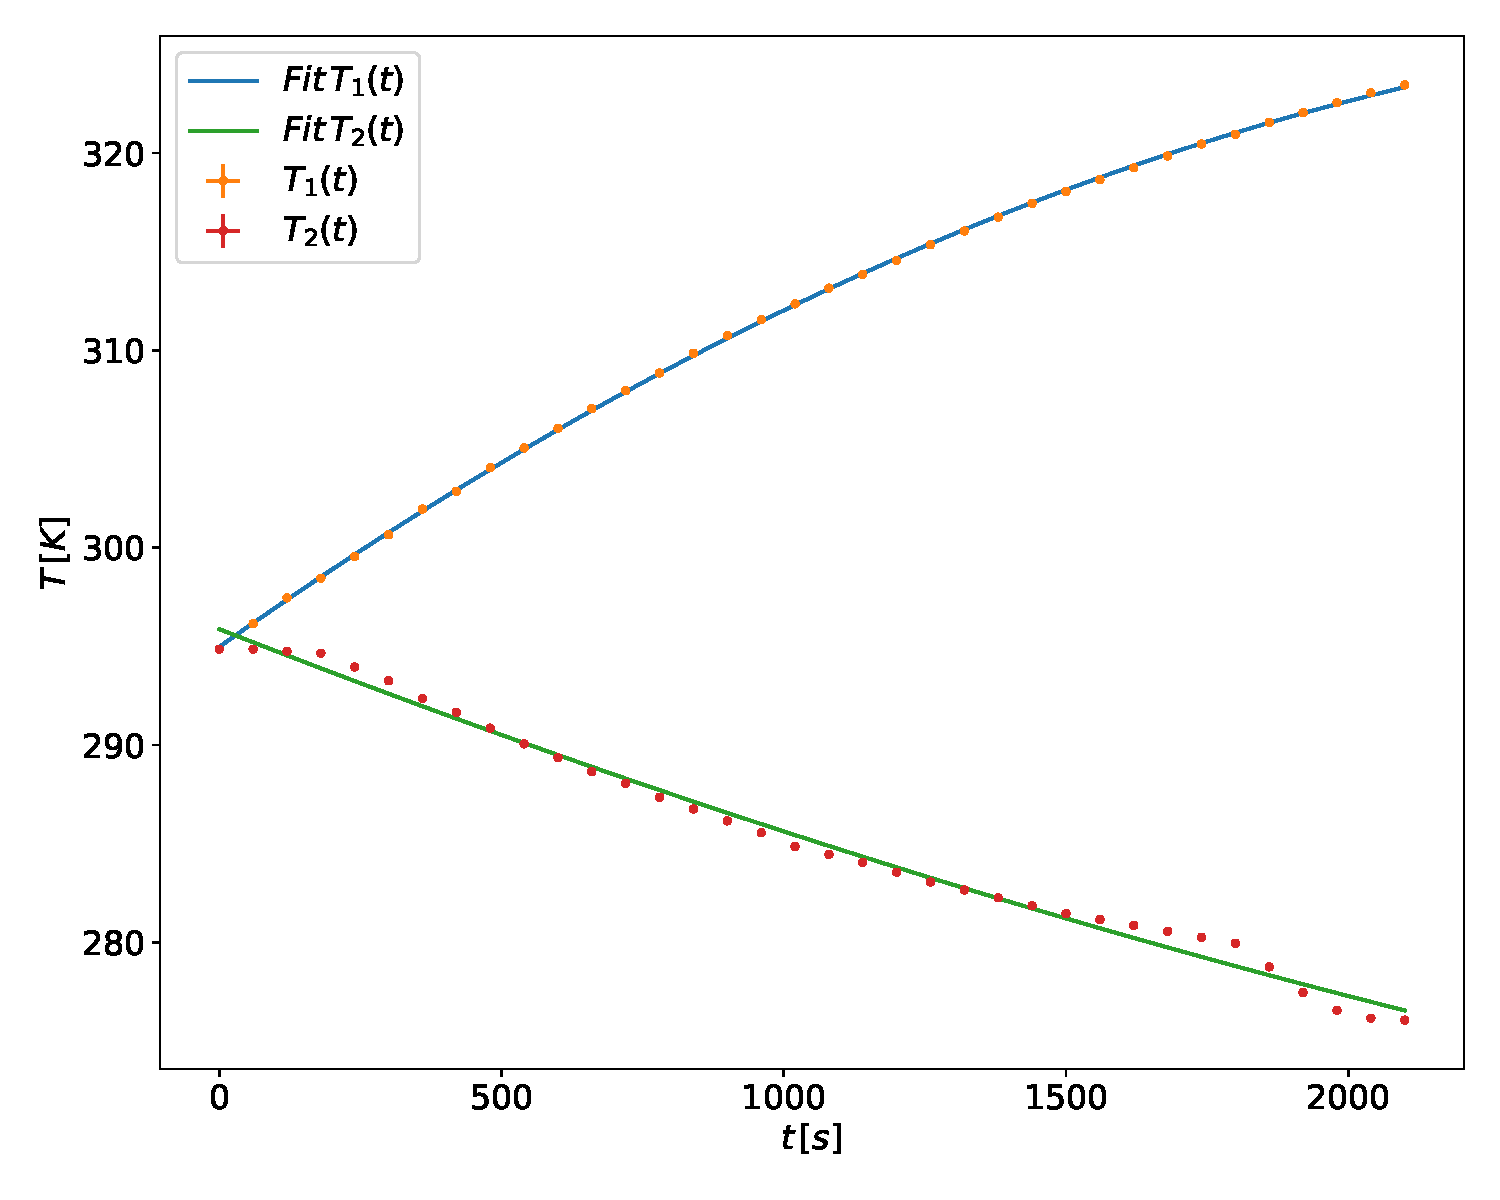
\includegraphics[width=\textwidth]{Daten/grafic.pdf}
    \caption{$U_\text{Br}$/ $U_\text{S}$ gegen $\omega/\omega_0$ aufgetragen. Theoretisch und gemessen.}
\end{figure}

In der Grafik sieht man das links vom Scheitel die Theoretischen und gemessen Werte relativ dicht beeinander liegen, jedoch die gemessenen Werte nicht am Scheitel 0 erreichen. Zusätzlich
sieht man das die Werte auf der rechten Seite anfangen wieder stark zu fallen, nachdem die gemessene Kurve anfängt abzuflachen. Die Gerade ab 5 kann durch den Mangel an Messpunkten
erklärt werden, da jeweils die Messpunkte durch eine direkte Verbindung verbunden wurden und keine Funktion durchgeplotet wurde.
Aus der Grafik lässt sich der Tiefpunkt der gemessene Tiefpunkt bei (1.0002|0.0141) ablesen. 
Daraus folgt dass das gemessene $\omega0 = 2356.19$. Dieser liegt sehr nah am theoretisch ermittelten Wert, $\omega0 = 2355.71$. 

Nun ist es möglich den Klirrfaktor nach (\ref{eqn:klirr}), (\ref{eqn:2oberwelle}) und (\ref{eqn:betragub}) aus der Messung zu bestimmen. Jedoch wird angenommen, 
dass die Summe der Oberwellen nur aus der zweiten Oberwelle besteht.

$U_2$ lässt sich durchschnittlich zu $U_2 = 12.299 \si{\volt}$ bestimmen. Daraus folgt ,mit $f(2) = 0.149$, dass der Klirrfaktor durchschnittlich $k = 12.2995$ betragen muss.
